\section{Monitor \& Controlling Process Group}
Ora dobbiamo controllare che il piano fin'ora sviluppato venga rispettato. Monitoraggio e controllo non sono sinonimi.
\begin{itemize}
	\item \textbf{Monitoraggio} significa raccogliere dati, i quali vengono utilizzati per verificare se il progetto sta venendo svolto nel modo corretto. Il piano, anche denominato "baseline" ci fornisce indicazioni su cosa significhi "modo corretto".
	\begin{info}
		Essere in baseline significa "star rispettando il piano" o "essere al passo col piano". Se un'attività per esempio sta venendo svolta in ritardo rispetto ad una tabella di marcia allora non siamo in baseline e bisogna cercare di recuperare;
	\end{info}
	\item Controllo significa fare qualcosa, ovvero portare una situazione in una fase accettabile secondo il piano. Non serve intervenire non appena si verifica un lieve ritardo. Esistono dei valori soglia che ci indicano quando conviene intervenire.  In alcuni casi il motivo dei ritardi è chiaro, in altri serve capire le cause per poter trovare le contromisure. Anche "non fare niente" è un'opzione accettabile a volte.
\end{itemize}

\subsection{Tools, templates e processi per monitorare e controllare il progetto}
La maggior parte dei tool nella fase di monitoraggio consiste in report.
\begin{itemize}
	\item \textbf{Current period reports}: focalizzati sul lavoro di un certo periodo di tempo corrente. Coprono solo i periodi più recenti del progetto. Evidenziano le attività completate più rilevanti e le eventuali variazioni rispetto a quanto pianificato. Possono anche includere un’analisi delle ragioni che hanno causato le eventuali variazioni e sulle corrispondenti misure correttive. In Scrum il periodo potrebbe essere anche il tempo di uno sprint. Sconsigliato un periodo troppo breve come "un giorno" perché l'overhead aumenta. Una base settimanale può essere un buon periodo;
	\item \textbf{Cumulative reports}: focalizzati sull'andamento del progetto (dall'inizio). Coprono l’intera storia del progetto e sono molto efficaci nel mostrare i trend nell’avanzamento del progetto. Per esempio, possono essere tracciati tutti gli scostamenti rispetto al pianificato e rilevare se la “situazione” sta migliorando o peggiorando;
	\item \textbf{Exception reports}: focalizzati principalmente su problemi o su attività problematiche. Sono rivolti al senior management e si concentrano sulla descrizione degli scostamenti rispetto al pianificato, delle cause e delle misure correttive da intraprendere. Sono molto sintetici e tuttalpiù prevedono degli allegati con maggiori dettagli;
	\item \textbf{Stoplight reports}: focalizzati per esempio sui colori, offrono un approccio visuale molto comodo per capire se si è in tempo con determinate attività oppure no. Possono essere visti come una variante applicata ai report
	di tipo current period, cumulative ed exception. Puntano a segnalare al senior management in modo estremamente sintetico lo stato di avanzamento del progetto. Per esempio, si può pensare di aggiungere agli altri tipi di report delle note con supporti visuali (e.g., post-it) per identificare rapidamente delle situazioni.
	\begin{info}[Esempio dell'utilizzo dei colori in stoplight]
		\item \textit{Verde}: “tutto procede come pianificato”;
		\item \textit{Giallo}: “vi sono stati scostamenti ma è tutto sotto controllo”;
		\item \textit{Rosso}: “situazione fuori controllo”. Una riunione in questo caso è quasi sempre necessaria;
	\end{info}
	Utilizzare pochi colori rende semplice capire le situazioni, aggiungerne rende più specifiche le situazioni ma rende più difficile l'identificazione rapida del problema;
	\item \textbf{Variance reports}: focalizzati sulle variazioni, sulle differenze. Concentrano la loro attenzione sugli scostamenti rispetto al pianificato. Per ogni attività e periodo riportano il confronto tra quanto pianificato e lo stato di avanzamento effettivo. Per riportare le informazioni possono essere utilizzate sia delle tabelle che dei grafici;
	\item \textbf{Gantt charts}: Durante questa fase diventa strumento di monitoraggio perché grazie è possibile capire la situazione delle attività attuale rispetto a quella prevista;
	\item \textbf{Burn charts}: Focalizzato su quanto lavoro manca. Si misura il lavoro come un "qualcosa che va bruciato", e si finisce quando tutto è stato bruciato;
	\item \textbf{Milestone trend charts}: Focalizzato sull'andamento delle milestone;
	\item \textbf{Earned value analysis}: Lo strumento sulla carta più quantitativo. C'è l'idea di cercare di capire quale valore stiamo recuperando. Verrà approfondito in seguito;
	\item \textbf{Integrated milestone trend charts and earned value analysis}: mix delle due precedenti soluzioni;
	\item \textbf{Project status meetings}: qualsiasi tipo di meeting è anche monitoraggio, dallo stand-up meeting al meeting di fine di uno sprint in scrum;
	\item \textbf{Problem escalation strategies}: un metodo di controllo in cui si chiede aiuto in "ordine gerarchico" fino a quando il problema non viene risolto. Per esempio il team prova a risolvere il problema prima di chiedere aiuto ad un livello più alto.
\end{itemize}
\subsubsection{Rispettare la Schedula di progetto}
Per mantenere il progetto entro i binari stabiliti in fase di pianificazione, secondo le buone pratiche è necessario:
\begin{itemize}
	\item \textbf{Tenere dei daily team meetings}: per riuscire a risolvere problemi prima che diventino troppo grandi per poter essere risolti efficacemente;
	\item \textbf{Completare i tasks il prima possibile};
	\item \textbf{Riportare eventuali problemi il prima possibile};
	\item \textbf{Non essere vittima delle “creeps”}: Ricordiamo che le creeps sono sono quei cambiamenti lievi ed impercettibili ed insidiosi, ma quando i loro effetti si accumulano possono diventare problemi importanti;
	\item \textbf{Non provare a indovinare: nel dubbio bisogna fare domande};
	\item \textbf{“Good enough is good enough”}: se non lavoriamo per avere eccellenza ma lavoriamo che fare in modo che tutto funzioni e basta il risultato finale sarà medio. Mantenere un passo costante e cercare di minimizzare il debito tecnico devono sempre essere questioni centrali;
	\item \textbf{Rispettare i requisiti, ma non andare oltre i requisiti (rischio di overdesign)}: overdesign significa aggiungere qualcosa di non richiesto o non gradito;
	\item \textbf{Bisogna essere aperti e onesti con i propri colleghi del team}: mentire significa sabotare il sistema di monitoraggio. Spesso si pensa che tenere nascosto qualcosa nella speranza che si risolva il prima possibile sia meglio che ammettere di essere in ritardo.
\end{itemize}

\subsection{Sistema di reporting}
\subsubsection{Effective Progress Reporting}
Per effettuare in modo efficiente il reporting sullo stato di avanzamento del progetto è consigliabile dotarsi di un sistema di supporto (Progress Reporting System), che dovrebbe avere le seguenti caratteristiche:
\begin{itemize}
	\item \textbf{Fornire informazioni sullo stato di avanzamento tempestive, complete e accurate}: uno dei problemi di sistemi di rendicontazioni è che inserire a fine orario di lavoro le entry su cosa è stato fatto durante la giornata non è divertente e spesso viene posticipato, causando problemi come la perdita di informazioni se non la completa assenza. Inoltre non avere inserimenti costanti non permette di fare monitoraggio costante, causando ritardi in processi di controllo;
	\item \textbf{Non deve richiedere un “overhead” eccessivo per il suo utilizzo (in termini di effort), tanto da essere controproducente}: sarebbe ideale avere un sistema di rendicontazione automatico ma è praticamente impossibile. Possibile invece è avere a disposizione un sistema reattivo e rapido da usare, anche perché utilizzare troppo tempo per la rendicontazione ne toglie al lavoro effettivo;
	\item \textbf{Il reporting deve essere intuitivo e facilmente accettabile da parte del team di progetto e del senior management}: la curba di apprendimento deve essere molto bassa, serve il clima aziendale adatto per capire che il tool viene utilizzato per aiutare e non per giudicare. Prima si trova il problema e prima si recupera;
	\item \textbf{Il sistema deve essere un efficace strumento per poter avere un allarme tempestivo (early warning) se ci fossero dei problemi a rispettare quanto pianificato}.
\end{itemize}
\subsubsection{Come e quali informazioni aggiornare}
\begin{enumerate}
	\item Prima di tutto bisogna determinare i periodi da monitorare (e.g., settimana) e per ognuno di questi bisogna definire in quale giorno e ora aggiornare le informazioni (e.g., un particolare giorno della settimana e un orario ben preciso). Parola chiave di questo processo è consistenza;
	\item Riportare il lavoro effettivamente svolto durante il periodo in esame in modo fedele;
	\item Registrare tutti i dati storici sull’eseguito nei periodi precedenti e aggiornare le stime sulle attività rimanenti. Utile per mantenere visione su cosa è stato fatto e cosa rimane da fare;
	\item Riportare le date di inizio e fine di ciascuna attività iniziata o terminata nel periodo in esame;
	\item Registrare i giorni già impegnati su ciascuna attività e quelli previsti per il completamento;
	\item Riportare le risorse consumate e quelle rimanenti;
	\item Riportare la percentuale di completamento. Problematico perché la "definizione di DONE" permette di capire bene quando un'attività è stata completata al 100\%, ma difficile fornire valori intermedi. Una possibilità è fornire un peso ad ogni test.
\end{enumerate}

\subsection{Strumenti di reporting visuale}

\subsubsection{Gantt Chart Project Status Report}
Ogni riga nel Gantt è un'attività. Ogni barra ci dice quando l'attività dovrebbe iniziare e quando dovrebbe finire. Nell'immagine che segue la linea tratteggiata indica il giorno corrente. Attraverso il sistema di rendicontazione è anche possibile avere un'indicazione proprio sul Gantt per capire come stanno andando le attività.
\centeredImage{document/img/ganttchart.png}{Gantt Chart Project Status Report}{0.6}

\subsubsection{Cumulative Reports - Milestone Trend Charts}
I Cumulative Report che seguono sono stati organizzati mettendo sulle ascisse i mesi di progetto. Se il puntino di ogni mese rimane su un valore di \textit{y} uguale a 0 allora siamo in schedula. Se il valore di \textit{y} è maggiore di 0, per esempio è 1, allora siamo in anticipo di un mese rispetto ai tempi. Se il valore di \textit{y} è sotto lo 0, ad esempio è -2, siamo in ritardo di due mesi. In questi cumulative report mancano informazioni sulle ragioni di anticipi e ritardi. Il Cumulative Report ci fornisce indicazioni su come sta andando il progetto rispetto al passato.\newline

\noindent Prendiamo in considerazione l'immagine \ref{cumreport1}. Capiamo facilmente che il progetto di questo cumulative report sta andando male, e i ritardi continuano ad aggiungersi. In questi casi bisogna assolutamente capire cosa non sta funzionando e perché. Un buon Project Manager avrebbe dovuto agire intorno al terzo o quarto mese. In alcuni casi questa situazione può anche essere tollerabile, ma devono esserci motivazioni valide.
\begin{figure}[H]
	\centering
	\begin{subfigure}[b]{0.45\textwidth}
		\centering
		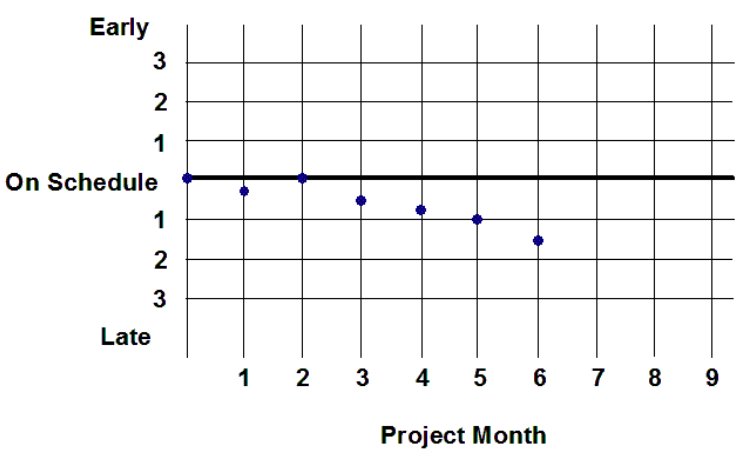
\includegraphics[width=\textwidth]{document/img/cumreport1.png}
		\caption{Cumulative Report \#1}
		\label{cumreport1}
	\end{subfigure}
	\hfill
	\begin{subfigure}[b]{0.45\textwidth}
		\centering
		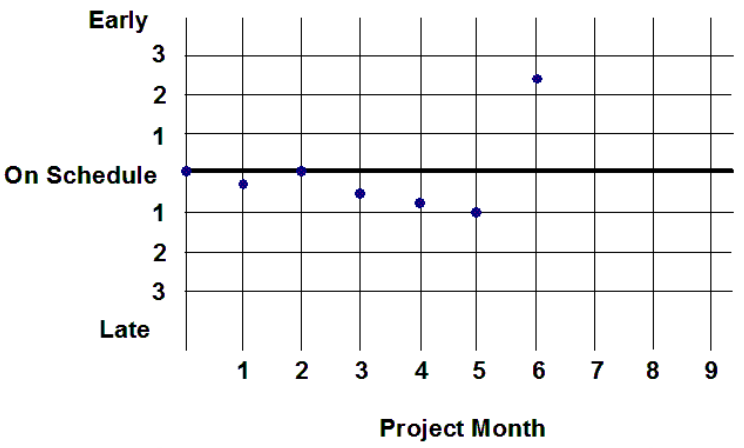
\includegraphics[width=\textwidth]{document/img/cumreport2.png}
		\caption{Cumulative Report \#2}
		\label{cumreport2}
	\end{subfigure}
	\caption{Esempi di Cumulative Reports}
\end{figure}

\noindent Nell'immagine \ref{cumreport2} invece nel giro di un mese la situazione è migliorata moltissimo. Questo può essere dovuto ad una contromisura come l'aggiunta di molto personale o la rimozione di molti requisiti. Una volta apportate le contromisure è stato rivalutato il piano. Secondo i nuovi parametri quindi lo stato di avanzamento del progetto è molto in anticipo. Guardando solo questo grafico la situazione dei ritardi sembra migliorata notevolmente, ma non sappiamo cosa è peggiorato per portarci a questa situazione. È sempre una questione di compromessi.\newline

\noindent Nell'immagine \ref{cumreport3} il progetto parte subito in anticipo dai primi mesi. In questo caso SOLO le attività del primo mese sono state valutate in modo pessimistico, infatti una volta portate a termine la situazione rimane abbastanza costante. Probabilmente si è preferito stare larghi probabilmente a causa di fattori di rischio (come una nuova tecnologia). Per il resto tutto sta procedendo come pianificato. Il mese guadagnato finisce nella scope bank.

\begin{figure}[H]
	\centering
	\begin{subfigure}[b]{0.45\textwidth}
		\centering
		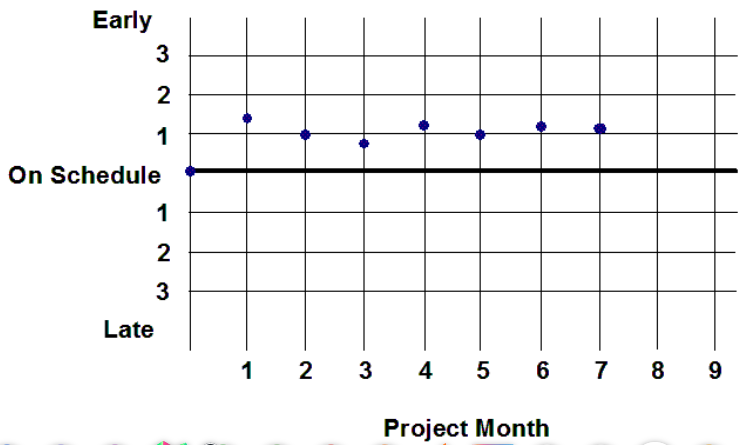
\includegraphics[width=\textwidth]{document/img/cumreport3.png}
		\caption{Cumulative Report \#3}
		\label{cumreport3}
	\end{subfigure}
	\hfill
	\begin{subfigure}[b]{0.45\textwidth}
		\centering
		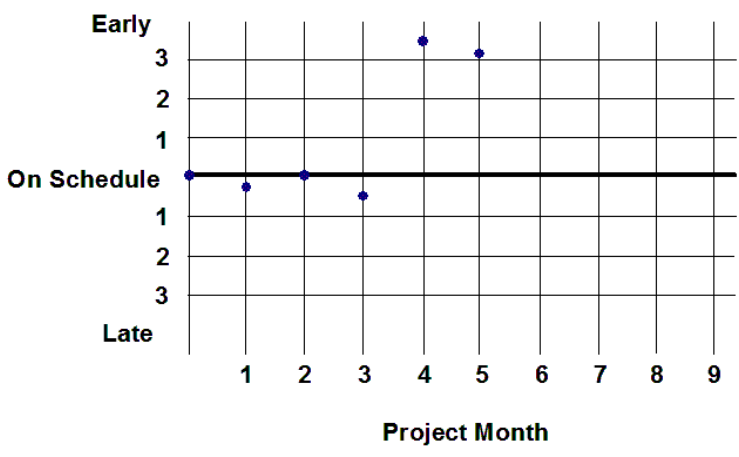
\includegraphics[width=\textwidth]{document/img/cumreport4.png}
		\caption{Cumulative Report \#4}
		\label{cumreport4}
	\end{subfigure}
	\caption{Altri esempi di Cumulative Reports}
\end{figure}

\subsection{Gestire la Scope Bank}
\subsection{Costruire e mantenere l’Issues Log}
\subsection{Gestire i Project Status Meetings}
\subsection{Definire una Problem Escalation Strategy}
\subsection{Acquisire l’approvazione a chiudere il progetto}
